%!TEX root = ../../thesis.tex
\section{Effects}
\label{sec:webaudio-effects}

\begin{quote}
  ``Anything more than three chords is just showing off.'' -
  Woody Guthrie
\end{quote}

In addition to filters (see \refchapter{sec:webaudio-filter}), there is a myriad of ways to shape sounds in order to create different effects. Two common techniques that can be used to create a variety of effects will be shown in this section: convolution and waveshaping.

\subsection{Convolution}

Convolution is most commonly used in audio programming for creating reverb effects. Reverb effects add the characteristics of locations to sounds. For example, by adding a reverb to the recording of a guitar chord, it can sound like it was recorded in a concert hall, a cave or under water. The base of this technique is the so-called Impulse Response (IR) which describes the characteristics of a system (here: the audio characteristics of a location) and its influence on an input signal \cite[p. 132ff]{park2009introductionto}. IRs are created by playing back a base audio signal (e.g. a clap) in a desired location. The playback is recorded and afterwards the original audio signal is deleted from the recording, so that only the room effect is left in the recording \cite[chapter: Room Effects]{smus2013webaudio}. In order to apply the IR to an arbitrary sound, the IR's signal is multiplied with the sound signal and the resulting signal contains the reverb effect. The mathematical model for this operation is convolution, which is why the effect is also often called convolution reverb\footnote{\cite[p. 139f]{park2009introductionto}}.

Convolution is a computationally intensive operation, thus it would result in a high CPU usage if done in JavaScript. The Web Audio API comes with a \code{ConvolverNode} \cite[chapter: ConvolverNode]{wilson2014webaudiospec}, which uses a C++ convolution engine under the hood to enable the computation in real-time\footnote{\url{https://chromium.googlesource.com/chromium/blink/+/32c15b00f4deb24f3f55156eba1c27fb506711d2/Source/modules/webaudio/ConvolverNode.cpp}, line 85, last checked on 19/03/2014}\footnote{Only Google Chrome's source is referenced here, but it is assumed that all other browser vendors also use a native engine for most Web Audio Nodes.}.

\begin{lstlisting}[language=JavaScript, caption=ConvolverNode usage, label=lst:convolver-node]
  var song = getSong("faith+1/01.mp3");
  var ir = getFile("reverb/church.wav");

  var convolver = context.createConvolver();
  convolver.buffer = ir;

  song.connect(convolver);
  convolver.connect(contxct.destination);
\end{lstlisting}

The above example (\reflisting{lst:convolver-node}) demonstrates the simple usage of the \code{ConvolverNode}. An IR is loaded from a file (line 2) and then assigned to the \code{buffer} of a newly created \code{ConvolverNode} (line 4f). Then, the \code{song} simply needs to be connected to the \code{convolver} (line 7) and the input signal is convolved with the IR's signal. The intense calculation is hidden and common Web Audio API patterns, like reusing buffers as IRs, are applied to make the \code{ConvolverNode} easy to use. In this case, the song playback would receive a hall effect similar to one that can be found in churches.

\subsection{Waveshaping}

Waveshaping is a technique to distort a sound signal. For this purpose, a shaping function is applied to an audio signal to shape the wave in a desired way \cite[p. 252]{curtis1996computer}.

\begin{figure}[htb]
  \centerline{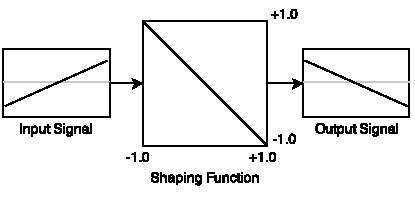
\includegraphics[width=0.75\linewidth]{images/waveshaping.pdf}}
  \caption[Using a waveshaping function to transform a signal -
  \protect\newline{\small based upon \cite[p. 255]{curtis1996computer}}]{Using a waveshaping function to transform a signal}
  \label{fig:waveshaping}
\end{figure}

The example in \reffigure{fig:waveshaping} shows a linear shaping function ($ f(x) = -x $) and a linear input signal. The output of the shaping function is an inverted input signal. For the purpose of simplicity, both, the input signal and the shaping function, are linear functions, but waveshaping is not limited to linear functions. In normal applications of waveshaping, the signal and the shaping function are non-linear. For faster computation, shape functions can be represented as in-memory look-up tables for values from -1 to 1. A typical application for waveshaping is the overdrive effect, which is well-known from the distorted sound of heavy guitar music.

In the Web Audio API there is a special node for waveshaping, the \code{Wave\allowbreak ShaperNode}. It uses a pre-stored wave function to shape the connected audio signal. The following example creates an overdrive effect and is taken from the \code{tuna} library\footnote{\url{https://github.com/Dinahmoe/tuna}, Dinahmoe, last checked on 20/03/2014}, which provides a variety of effects for the Web Audio API\footnote{For abbreviation, the part about loading and connecting a buffer, as seen in the examples before, is left out.}.

\begin{lstlisting}[language=JavaScript, caption=Using the WaveShaperNode, label=lst:waveshaper-node]
  var samples = 8192;
  var table = new Float32Array(samples);
  var amount = .7;
  var k = 2 * amount / (1 - amount),
      i, x;
  for(i = 0; i < samples; i++) {
    x = i * 2 / samples - 1;
    table[i] = (1 + k) * x / (1 + k * Math.abs(x));
  }

  waveshaper = context.createWaveShaper();
  waveshaper.curve = table;
\end{lstlisting}

For the representation of the curve, a \code{Float32Array} is used instead of a normal array (line 2, \reflisting{lst:waveshaper-node}), which is filled by iterating over the amount of \code{samples} (line 6) and calculating the function's value at the current point (line 8). In short, the above created curve table represents a variable version of the mathematical function $ f(x) = \frac{x}{abs(x)} $ which acts as a clipping function for the input signal. The clipping threshold is defined by the value of \code{amount} (line 3) and is typically a parameter that is defined by users.